\section {Pigsty for six pigs (Geometry)}
A farmer has obtained $13$ panels in order to create 6 identical pigsties. He was planning to arrange them like this:

\begin{center}
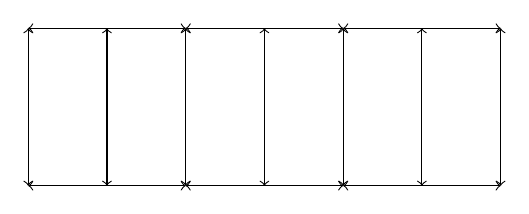
\begin{tikzpicture}[scale=2]

\draw [<->] (0,0) -- (1,0);
\draw [<->] (1,0) -- (2,0);
\draw [<->] (2,0) -- (3,0);

\draw [<->] (0,1) -- (1,1);
\draw [<->] (1,1) -- (2,1);
\draw [<->] (2,1) -- (3,1);

\draw [<->] (0.0,0) -- +(0,1);
\draw [<->] (0.5,0) -- +(0,1);
\draw [<->] (1.0,0) -- +(0,1);
\draw [<->] (1.5,0) -- +(0,1);
\draw [<->] (2.0,0) -- +(0,1);
\draw [<->] (2.5,0) -- +(0,1);
\draw [<->] (3.0,0) -- +(0,1);

\end{tikzpicture}
\end{center}

Unfortunately, one of his panels got stolen and he now only has $12$ panels. Can you design $6$ identical pigsties with $12$ panels?

\subsection{Solution}

\begin{center}
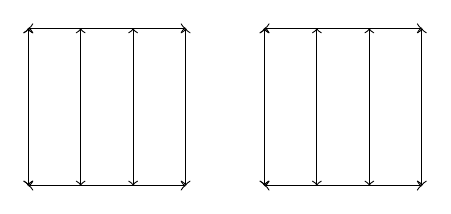
\begin{tikzpicture}[scale=2]

\draw [<->] (0,0) -- +(1,0);
\draw [<->] (0,0) -- +(0,1);
\draw [<->] (1,0) -- (1,1);
\draw [<->] (0,1) -- (1,1);

\draw [<->] (0.0,0) -- +(0,1);
\draw [<->] (0.333,0) -- +(0,1);
\draw [<->] (0.666,0) -- +(0,1);

\draw [<->] (1.5,0) -- +(1,0);
\draw [<->] (1.5,0) -- +(0,1);
\draw [<->] (1.5,1) -- +(1,0);
\draw [<->] (2.5,0) -- +(0,1);

\draw [<->] (1.5,0) -- +(0,1);
\draw [<->] (1.833,0) -- +(0,1);
\draw [<->] (2.166,0) -- +(0,1);
\end{tikzpicture}
\end{center}
